\section{Problem Formulation}
\label{sec:problem}

This section fixes the vocabulary used in the rest of the paper. \Cref{tab:notation} lists the main symbols.

\subsection{Executable business specifications}

\begin{definition}[Executable business specification]
\label{def:spec}
An \emph{executable business specification} is a triple $\Spec=\langle\Tell,\Chk,\Scen\rangle$, where:
\begin{itemize}[leftmargin=*]
\item $\Tell$, the \emph{Tell} part, is everything an executor is told. In our subject these are the requirement documents, knowledge-base articles, business principles, tool catalogue, database schema, scope table and the refusal messages returned by tools.
\item $\Chk=\{\varphi_1,\dots,\varphi_{|\Chk|}\}$, the \emph{Check} part, is a finite set of clauses that can be evaluated on a behaviour. These are invariants, expectations, golden-state values, guardrails, blank-column rules and event vocabulary.
\item $\Scen$ is the scenario space. A scenario $\pi\in\Scen$ is a vector of task parameters, such as the ordered quantity, the received quantity, the requested discount and the number of receipts per order.
\end{itemize}
\end{definition}

We deliberately exclude any hand-written ``playbook'' that explains how to carry out the process. A playbook is one human's interpretation of $\Tell$. Including it would test the playbook, not the specification.

\paragraph{Behaviours.} A run of an executor on scenario $\pi$ produces a \emph{behaviour} $b$. It consists of the rows the run committed to the database, the events it logged, the tool calls the guardrails refused and the executor's final claim. Each clause is a function
\begin{equation}
\label{eq:eval}
\varphi:\Beh\to\{\sat,\viol,\na\},
\end{equation}
where $\na$ means that the clause does not apply, for instance because the rows it reads do not exist in $b$. We write $b\models\varphi$ when $\varphi(b)=\sat$, and $b\models\Chk'$ when $b\models\varphi$ for every applicable $\varphi\in\Chk'$. The \emph{violation set} of $b$ is
\begin{equation}
\label{eq:violset}
V(b)=\{\varphi\in\Chk:\varphi(b)=\viol\}.
\end{equation}

\paragraph{Clause lifting.} Many clauses state facts of one reference case as literals, such as ``the ordered quantity equals 15''. \emph{Lifting} rewrites such a clause into a form that depends on the scenario, here $\textit{ordered}=\pi.\textit{ordered}$. It does so by anti-unifying the clause's literals with the parameters of the reference scenarios. A literal is lifted only when it matches the same parameter in every reference scenario; otherwise the clause stays bound to the scenario it came from. We write $\Chk(\pi)$ for the lifted clauses that apply in $\pi$.

\paragraph{Specification-induced equivalence.} Two behaviours may differ in ways the specification does not care about, such as timestamps, serial identifiers or free text. The relation $\equiv_\Spec$ compares behaviours only on the \emph{locked} columns: keys, statuses, quantities, approvals and the $(\textit{kind},\textit{ref},\textit{actor})$ of events. It also requires the \emph{blank} columns to be null in both behaviours. The classification of every column is derived automatically from the schema and the specification's metadata, so the specification itself, and not the researcher, decides what counts as ``the same outcome''.

\subsection{Interpreters and admissible behaviours}

An \emph{interpreter} $I$ maps $(\Tell,\pi)$ to a behaviour at random. An interpreter is a model $m$ together with a Tell variant $v$ and a sampling seed $r$. The ideal interpreter $I^\star$ produces exactly the behaviours that $\Tell$ permits,
\begin{equation}
\label{eq:adm}
\Adm_\Tell(\pi)\subseteq\Beh .
\end{equation}
$\Adm_\Tell(\pi)$ is never observed directly; it is the object that \specdx estimates. A population $\Pop=\{(m,v,r)\}$ draws from $\Models\times\{0,1,2\}\times\{1,2,3\}$. Variant 0 is the original text. Variants 1 and 2 paraphrase only the standing instruction and the task statement, so that a seeded ambiguity in the retrieved requirements is not washed out.

\subsection{Defect taxonomy}

Each defect type is defined purely by satisfaction on a scenario $\pi$.

\begin{definition}[Defect types]
\label{def:defects}
Let $\pi\in\Scen$.
\begin{enumerate}[leftmargin=*,label=(\roman*)]
\item \textbf{Contradiction.} A set $M\subseteq\Chk(\pi)$ is a contradiction when no behaviour satisfies it:
  \begin{equation}\label{eq:def-con}
  \nexists\,b\in\Beh:\;b\models M .
  \end{equation}
  It is reported as a minimal unsatisfiable subset (MUS).
\item \textbf{Hidden requirement.} A clause $\varphi$ is a hidden requirement when some admissible behaviour satisfies every other clause but not $\varphi$:
  \begin{equation}\label{eq:def-hid}
  \exists\,b\in\Adm_\Tell(\pi):\;b\models\Chk(\pi)\setminus\{\varphi\}\;\wedge\;b\not\models\varphi .
  \end{equation}
  Here $\Chk$ is stricter than $\Tell$ at $\varphi$.
\item \textbf{Ambiguity.} $\Tell$ is ambiguous at $\pi$ when it admits more than one outcome up to $\equiv_\Spec$:
  \begin{equation}\label{eq:def-amb}
  \bigl|\Adm_\Tell(\pi)/{\equiv_\Spec}\bigr|\ge 2 .
  \end{equation}
  It is located at the sentences of $\Tell$ responsible for the split.
\item \textbf{Weak check.} $\Chk$ is weak at $\pi$ when a behaviour that $\Tell$ forbids passes every check:
  \begin{equation}\label{eq:def-weak}
  \exists\,b\notin\Adm_\Tell(\pi):\;b\models\Chk(\pi) .
  \end{equation}
  Here $\Chk$ is looser than $\Tell$. The defect is located at the locked field on which $b$ departs from the admissible outcomes.
\end{enumerate}
\end{definition}

\Cref{fig:taxonomy} pictures the four definitions as relations between two sets of behaviours: those that $\Tell$ admits and those that pass the checks.

\begin{figure}[t]
\centering
\resizebox{\textwidth}{!}{% Defect taxonomy as relations between the admissible behaviours and the behaviours that pass the checks.
\begin{tikzpicture}[
  every node/.style={font=\footnotesize},
  adm/.style={draw=blue!60!black, fill=blue!12, fill opacity=0.8, text opacity=1},
  sat/.style={draw=orange!80!black, fill=orange!18, fill opacity=0.65, text opacity=1},
  beh/.style={draw=gray, rounded corners=2pt},
  pt/.style={circle, fill=black, inner sep=1.3pt}]
\foreach \x/\t in {0/{(a) Contradiction}, 3.55/{(b) Hidden requirement}, 7.1/{(c) Ambiguity}, 10.65/{(d) Weak check}} {
  \draw[beh] (\x,0) rectangle ++(3.25,2.6);
  \node[anchor=north west, gray] at (\x,2.6) {$\Beh$};
  \node[anchor=north, font=\footnotesize\bfseries] at (\x+1.625,-0.05) {\t};
}
% (a) no behaviour satisfies M
\draw[adm] (0.95,1.35) ellipse (0.7 and 0.55); \node at (0.95,1.35) {$\Adm_\Tell$};
\draw[draw=red!70!black, dashed, thick] (2.45,1.5) circle (0.4);
\draw[red!70!black, thick] (2.17,1.22) -- (2.73,1.78) (2.17,1.78) -- (2.73,1.22);
\node[red!70!black, align=center, font=\scriptsize] at (1.85,0.4) {no $b$ with $b\models M$};
% (b) an admissible behaviour fails one clause
\begin{scope}[shift={(3.55,0)}]
\draw[sat] (2.0,1.3) ellipse (1.05 and 0.8); \node at (2.45,1.75) {$\textsf{Sat}(\Chk)$};
\draw[adm] (1.05,1.2) ellipse (0.8 and 0.6); \node at (0.95,1.45) {$\Adm_\Tell$};
\node[pt] (b) at (0.6,1.0) {}; \node[font=\scriptsize, align=center] at (1.62,0.3) {$b\models\Chk\setminus\{\varphi\}$, $b\not\models\varphi$};
\end{scope}
% (c) two admissible classes
\begin{scope}[shift={(7.1,0)}]
\draw[adm] (1.62,1.3) ellipse (1.25 and 0.75);
\draw[blue!60!black, dashed] (1.62,0.55) -- (1.62,2.05);
\node at (1.05,1.3) {$[b_1]$}; \node at (2.2,1.3) {$[b_2]$};
\node[font=\scriptsize] at (1.62,0.3) {$|\Adm_\Tell/{\equiv_\Spec}|\ge2$};
\end{scope}
% (d) a non-admissible behaviour passes every check
\begin{scope}[shift={(10.65,0)}]
\draw[sat] (1.62,1.4) ellipse (1.3 and 0.85); \node at (2.35,1.95) {$\textsf{Sat}(\Chk)$};
\draw[adm] (1.25,1.25) ellipse (0.65 and 0.45); \node at (1.25,1.25) {$\Adm_\Tell$};
\node[pt] at (2.45,0.95) {}; \node[font=\scriptsize] at (1.62,0.22) {$b\notin\Adm_\Tell$, $b\models\Chk$};
\end{scope}
\end{tikzpicture}
}
\caption{The four defect types as relations between the admissible behaviours $\Adm_\Tell$ and the behaviours that pass the checks, $\textsf{Sat}(\Chk)$, inside the space of behaviours $\Beh$. (a)~No behaviour satisfies a clause set $M$. (b)~An admissible behaviour fails exactly one clause. (c)~The admissible behaviours fall into two classes of $\equiv_\Spec$. (d)~A behaviour outside $\Adm_\Tell$ passes every check.}
\label{fig:taxonomy}
\end{figure}

The types may co-occur. When $\Tell$ is ambiguous and $\Chk$ picks one of the readings, both an ambiguity and a hidden requirement are reported: the behaviours that follow the other reading satisfy \eqref{eq:def-hid}.

The definitions show why no single source of evidence is enough. A contradiction~\eqref{eq:def-con} concerns $\Chk$ alone. Sampling can never prove that no behaviour exists, so a contradiction can only be supported by failed attempts and refuted by a witness. A hidden requirement~\eqref{eq:def-hid} and an ambiguity~\eqref{eq:def-amb} quantify over $\Adm_\Tell$, which only an interpreter of $\Tell$ can sample. A weak check~\eqref{eq:def-weak} quantifies over behaviours \emph{outside} $\Adm_\Tell$, which an ideal interpreter never produces. Its detection therefore relies on interpreters that err. The following proposition makes the role of ideal interpreters precise.

\begin{proposition}[Soundness under ideal interpreters]
\label{prop:ideal}
Suppose every observed behaviour on $\pi$ is drawn from $\Adm_\Tell(\pi)$.
\begin{enumerate}[leftmargin=*,label=(\alph*)]
\item If an observed $b$ has $V(b)=\{\varphi\}$, then $\varphi$ is a hidden requirement. Whether $\varphi$ is also unsatisfiable on its own, a contradiction of size one, is left to refutation.
\item If two observed behaviours are not $\equiv_\Spec$-equivalent, then $\Tell$ is ambiguous at $\pi$.
\item If every clause is invariant under $\equiv_\Spec$ and the sample covers every class of $\Adm_\Tell(\pi)/{\equiv_\Spec}$, both tests are complete.
\end{enumerate}
\end{proposition}
The proof is in \cref{app:proofs}. Real interpreters are not ideal: they err, abstain, and err in correlated ways. The rest of the method is about recovering conclusions (a)--(c) when the observed behaviours mix admissible readings with interpreter errors.

\subsection{Cells: the unit of evidence}
\label{sec:cells}

Comparing whole behaviours is too coarse. Independent variation in several fields multiplies into many distinct outcomes, and nearly every pair of runs differs somewhere. \specdx therefore reads every behaviour at the level of \emph{cells}. We first define items.

\paragraph{Items.} An \emph{item} $s=(\pi,\textit{step})$ is one interpreter step of the process in a scenario.

\paragraph{Cells.} A \emph{cell} is the smallest unit of reading. There are two kinds.
\begin{itemize}[leftmargin=*]
\item A \emph{value cell} is a locked (table, row, column) triple, or one golden event $(\textit{kind},\textit{ref},\textit{actor})$. Its reading $y_{b,c}$ is the normalised value of the field in $b$'s end state, or \textsf{absent}.
\item A \emph{constraint cell} is one cross-cutting clause evaluated at an item. Its reading is $\sat$ or $\viol$.
\end{itemize}

\paragraph{Anchors.} The \emph{anchor} $d_c$ of a cell is what $\Chk$ declares for it: the (lifted) golden value of a value cell, \textsf{present} for a golden event, and $\sat$ for a constraint cell. A value cell on which $\Chk$ declares nothing is \emph{unanchored}. Unanchored cells contribute no evidence about accuracy, but they are where weak checks show up.

\paragraph{Pooling.} A lifted cell is one cell across all the scenarios where it applies. Its readings are pooled in the lifted vocabulary: a reading that equals the scenario's value of the parameter \textit{qty} is recorded as the placeholder \texttt{\{qty\}} in every scenario. Pooling increases the number of readings per cell, which the finite-sample bounds of \cref{sec:theory} depend on.

\Cref{fig:cells} shows what the data look like: a matrix of behaviours by cells, with the anchors in the first row and gaps where a behaviour did not act.

\begin{figure}[t]
\centering
\resizebox{0.95\textwidth}{!}{% From runs to cell readings: an illustrative reading matrix.
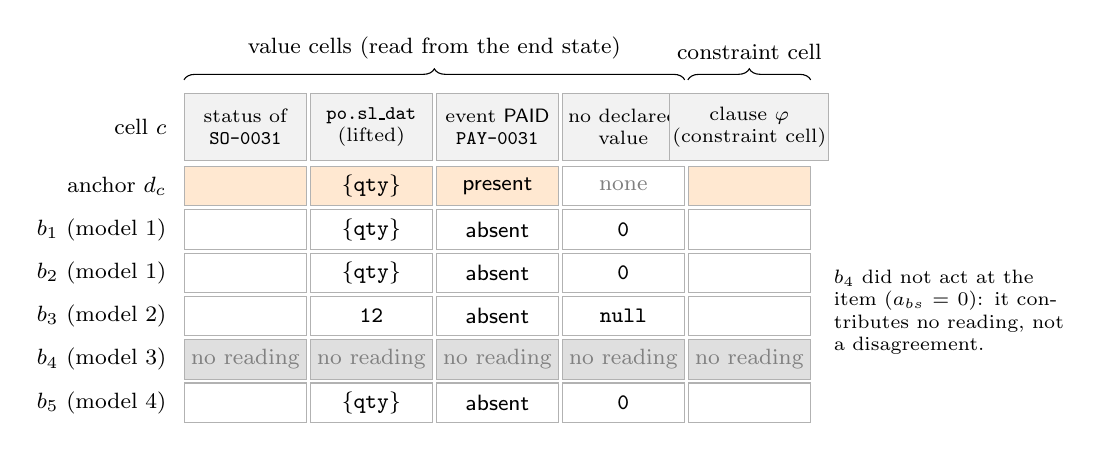
\begin{tikzpicture}[
  every node/.style={font=\footnotesize},
  cell/.style={draw=gray!60, minimum width=1.55cm, minimum height=0.5cm, inner sep=1pt},
  hd/.style={cell, fill=gray!10, font=\scriptsize, align=center, minimum height=0.85cm},
  an/.style={cell, fill=orange!18},
  miss/.style={cell, fill=gray!25, text=gray}]
\def\W{1.6}
% header
\node[anchor=east] at (-0.88,0.4) {cell $c$};
\foreach \i/\h in {0/{status of\\\texttt{SO-0031}}, 1/{\texttt{po.sl\_dat}\\(lifted)}, 2/{event \textsf{PAID}\\\texttt{PAY-0031}}, 3/{no declared\\value}, 4/{clause $\varphi$\\(constraint cell)}}
  \node[hd] at (\i*\W,0.4) {\h};
\node[anchor=east] at (-0.88,-0.35) {anchor $d_c$};
\foreach \i/\v in {0/{\viCho}, 1/{\texttt{\{qty\}}}, 2/{\textsf{present}}, 4/{\sat}}
  \node[an] at (\i*\W,-0.35) {\v};
\node[cell, fill=white, text=gray] at (3*\W,-0.35) {none};
% readings
\foreach \r/\lab/\va/\vb/\vc/\vd/\ve in {
  1/{$b_1$ (model 1)}/{\viDa}/{\texttt{\{qty\}}}/{\textsf{absent}}/{\texttt{0}}/{\sat},
  2/{$b_2$ (model 1)}/{\viCho}/{\texttt{\{qty\}}}/{\textsf{absent}}/{\texttt{0}}/{\viol},
  3/{$b_3$ (model 2)}/{\viDa}/{\texttt{12}}/{\textsf{absent}}/{\texttt{null}}/{\sat},
  4/{$b_4$ (model 3)}/{--}/{--}/{--}/{--}/{--},
  5/{$b_5$ (model 4)}/{\viDa}/{\texttt{\{qty\}}}/{\textsf{absent}}/{\texttt{0}}/{\sat}} {
  \node[anchor=east] at (-0.88,-0.35-0.55*\r) {\lab};
  \ifnum\r=4
    \foreach \i in {0,...,4} \node[miss] at (\i*\W,-0.35-0.55*\r) {no reading};
  \else
    \node[cell] at (0,-0.35-0.55*\r) {\va};
    \node[cell] at (\W,-0.35-0.55*\r) {\vb};
    \node[cell] at (2*\W,-0.35-0.55*\r) {\vc};
    \node[cell] at (3*\W,-0.35-0.55*\r) {\vd};
    \node[cell] at (4*\W,-0.35-0.55*\r) {\ve};
  \fi
}
% braces
\draw[decorate, decoration={brace, amplitude=4pt}] (-0.78,1.0) -- (3*\W+0.78,1.0) node[midway, above=4pt] {value cells (read from the end state)};
\draw[decorate, decoration={brace, amplitude=4pt}] (4*\W-0.78,1.0) -- (4*\W+0.78,1.0) node[midway, above=4pt, align=center] {constraint cell};
\node[anchor=west, align=left, font=\scriptsize, text width=3.0cm] at (4*\W+0.95,-1.95) {$b_4$ did not act at the item ($a_{bs}=0$): it contributes no reading, not a disagreement.};
\end{tikzpicture}
}
\caption{From runs to cell readings (illustrative values). Each row is one behaviour, each column one cell; the first row holds the anchors that $\Chk$ declares. Value cells are read from the end state, and a constraint cell is read as $\sat$ or $\viol$. A behaviour that did not act at the item contributes no reading.}
\label{fig:cells}
\end{figure}

The interpretation of a cell under each defect type follows from \cref{def:defects}. Let $A_c$ be the set of readings of $c$ that $\Tell$ admits. Then:
\begin{itemize}[leftmargin=*]
\item $A_c=\{d_c\}$ means no defect at $c$;
\item $d_c\notin A_c\neq\emptyset$ means a hidden requirement whose anchor is wrong (the \emph{mis-key} subtype);
\item $|A_c|=2$ means an ambiguity; when it contains $d_c$, $\Chk$ has picked one of the readings (the \emph{ambiguous-pick} subtype);
\item $A_c=\emptyset$ on an anchored cell means $\Tell$ says nothing about the cell while $\Chk$ fixes it (the \emph{unstated} subtype).
\end{itemize}
The subtypes are all hidden requirements in the sense of \eqref{eq:def-hid}, and they are reported as such.

\subsection{Problem statement}

\begin{quote}
\emph{Given} a specification $\Spec=\langle\Tell,\Chk,\Scen\rangle$, a population of local LLM interpreters $\Pop$ and a budget $B$ of runs, \emph{report} a ranked list of defects. Each defect carries a type from \cref{def:defects}, a location (a clause set, a clause, a set of sentences of $\Tell$, or a locked field), witness behaviours and a score. No human labels may be used.
\end{quote}

\begin{table}[t]
\caption{Main notation.}
\label{tab:notation}
\small
\begin{tabular}{@{}ll@{}}
\toprule
Symbol & Meaning \\
\midrule
$\Spec=\langle\Tell,\Chk,\Scen\rangle$ & Specification: Tell part, Check part (clauses $\varphi$), scenario space \\
$b$, $V(b)$ & Behaviour; its set of violated clauses \\
$\Adm_\Tell(\pi)$ & Behaviours that $\Tell$ permits in scenario $\pi$ \\
$m\in\Models$, $(m,v,r)\in\Pop$ & Model; interpreter (model, Tell variant, seed) \\
$s$, $a_{bs}$ & Item (scenario, step); act indicator \\
$\eta_m$, $\delta_s$, $O_s$ & Capability to act, item difficulty, observability (stage 1) \\
$c\in\Cells$, $d_c$, $V_c$ & Cell, its anchor, its candidate values (with \other) \\
$A_c\in\Sets_c$ & Latent set of admissible readings of $c$ \\
$\alpha_m$, $\beta_g$, $p_{m,c}$ & Model ability, group difficulty, accuracy $\sigma(\alpha_m-\beta_{g(c)})$ \\
$\varepsilon_c$, $\kappa$, $u_c$ & Error distribution, its concentration and flat pool \\
$r_{bc}$, $w_b$ & Probability that a reading is faithful; behaviour weight \\
$\tau_H,\tau_A,\tau_W$ & Typing thresholds (hidden, ambiguity, weak) \\
\bottomrule
\end{tabular}
\end{table}
